\documentclass[border=10pt]{standalone}
\usepackage{tikz}
\usetikzlibrary{shapes.geometric, arrows.meta, positioning}

\begin{document}
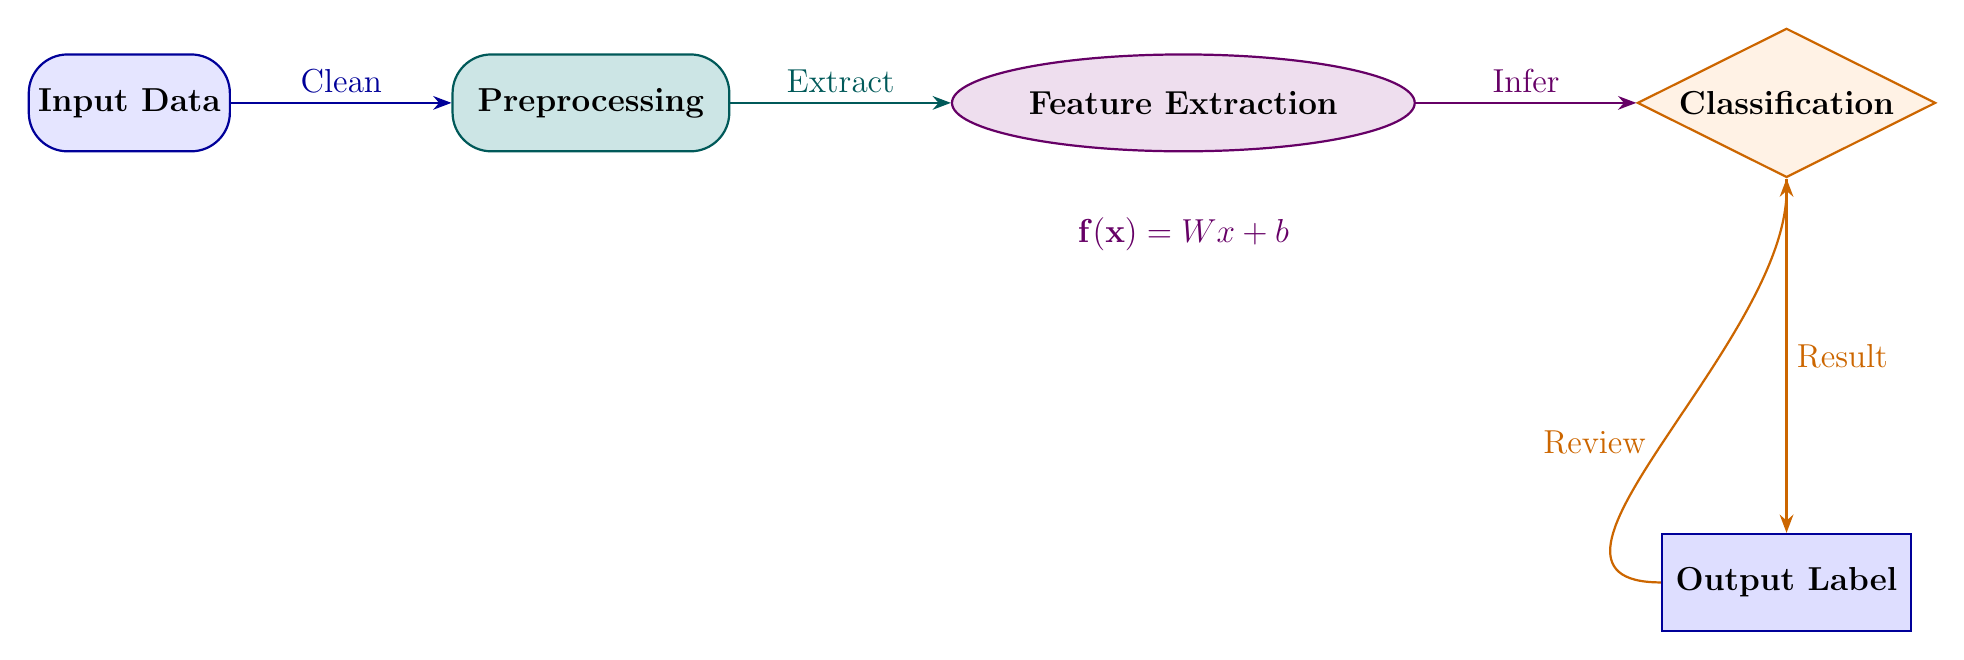
\begin{tikzpicture}[
    node distance=1.5cm and 2.8cm,
    % Styles for the nodes
    base/.style={draw, thick, minimum height=3.5em, text centered, font=\large\bfseries},
    input/.style={base, rectangle, rounded corners=1.4em, fill=blue!10, draw=blue!60!black, minimum width=7em},
    preproc/.style={base, rectangle, rounded corners=1.4em, fill=teal!20, draw=teal!70!black, minimum width=10em},
    feature/.style={base, ellipse, fill=violet!13, draw=violet!80!black, minimum width=13em},
    class/.style={base, diamond, aspect=2, fill=orange!10, draw=orange!80!black, minimum width=9em, inner xsep=0pt},
    output/.style={base, rectangle, fill=blue!13, draw=blue!60!black, minimum width=9em},
    % Style for the arrows
    arrow/.style={-Stealth, thick},
    % Style for the labels on arrows
    label/.style={font=\large}
]

% Place the nodes
\node (input) [input] {Input Data};
\node (preproc) [preproc, right=of input] {Preprocessing};
\node (feature) [feature, right=of preproc] {Feature Extraction};
\node (class) [class, right=of feature] {Classification};
\node (output) [output, below=4.5cm of class] {Output Label};

% Place the formula
\node (formula) [below=0.7cm of feature, text=violet!80!black, font=\large] {$\mathbf{f(x)} = Wx + b$};

% Draw the arrows and labels
\draw [arrow, blue!60!black] (input) -- (preproc) node [midway, above, label, text=blue!60!black] {Clean};
\draw [arrow, teal!70!black] (preproc) -- (feature) node [midway, above, label, text=teal!70!black] {Extract};
\draw [arrow, violet!80!black] (feature) -- (class) node [midway, above, label, text=violet!80!black] {Infer};
\draw [arrow, orange!80!black] (class.south) -- (output.north) node [midway, right, label, text=orange!80!black] {Result};

% Draw the review loop
\draw [arrow, orange!80!black] (output.west) to[out=180, in=270, looseness=1.0] node [midway, left, label, text=orange!80!black, xshift=-2pt] {Review} (class.south);

\end{tikzpicture}
\end{document}
